\documentclass[twoside,11pt]{article}

\usepackage{aa228-jmlr2e}
\usepackage{lipsum}
\usepackage{listings}
\usepackage{graphicx}
\usepackage{amsmath}
\usepackage{booktabs}
\usepackage{xcolor}
\usepackage{algorithm}

% Define Python syntax highlighting
\lstdefinestyle{pythonstyle}{
    language=Python,
    basicstyle=\ttfamily\small,
    commentstyle=\color{gray},
    keywordstyle=\color{blue},
    stringstyle=\color{red},
    numberstyle=\tiny\color{gray},
    numbers=left,
    numbersep=5pt,
    frame=single,
    breaklines=true,
    showstringspaces=false,
    tabsize=4
}

\begin{document}

% Refer to this link for project rubric: https://aa228.stanford.edu/project-1/
\title{Project 1: Bayesian Structure Learning}

%===========================================
% TODO: Replace "First Last" with your name.
% TODO: Replace "email@stanford.edu" with your Stanford email.
%===========================================
\name{Christopher Luey}
\email{luey@stanford.edu}


\maketitle

\section{Algorithm Description}
%===========================================
% TODO: Replace this with a short description of your algorithm(s) used.
This project implements a comprehensive Bayesian network structure learning system that combines multiple search heuristics to maximize the Bayesian Dirichlet equivalent uniform (BDeu) score with a Dirichlet(1) prior. The implementation uses an ensemble approach where three distinct algorithms are run sequentially, each seeded with the best results from prior searches.

The core scoring mechanism uses the BDeu metric with uniform Dirichlet prior ($\alpha_{ijk} = 1$). To improve scalability, the implementation employs mutual information-based parent candidate selection, reducing the search space from $O(n^2)$ to $O(nk)$ without significantly impacting solution quality.

The multi-algorithm ensemble consists of: (1) Hill Climbing with Tabu Search using greedy hill climbing with multiple random restarts and tabu memory to escape local optima, (2) Simulated Annealing using Metropolis-Hastings sampling with exponential temperature cooling to allow temporary moves to lower-scoring regions, and (3) Genetic Algorithm using edge-recombination with tournament selection, crossover, and mutation operators, seeded with the best solutions from previous phases.

The DAG representation uses adjacency matrices with efficient cycle detection via depth-first reachability checks. All local scores are maintained incrementally, avoiding redundant re-computation. The system automatically scales hyperparameters based on problem size.
%===========================================


\section{Graphs}
%===========================================
% TODO: Add your small, medium, and large graph visualizations here
%===========================================
\begin{figure}[h]
    \centering
    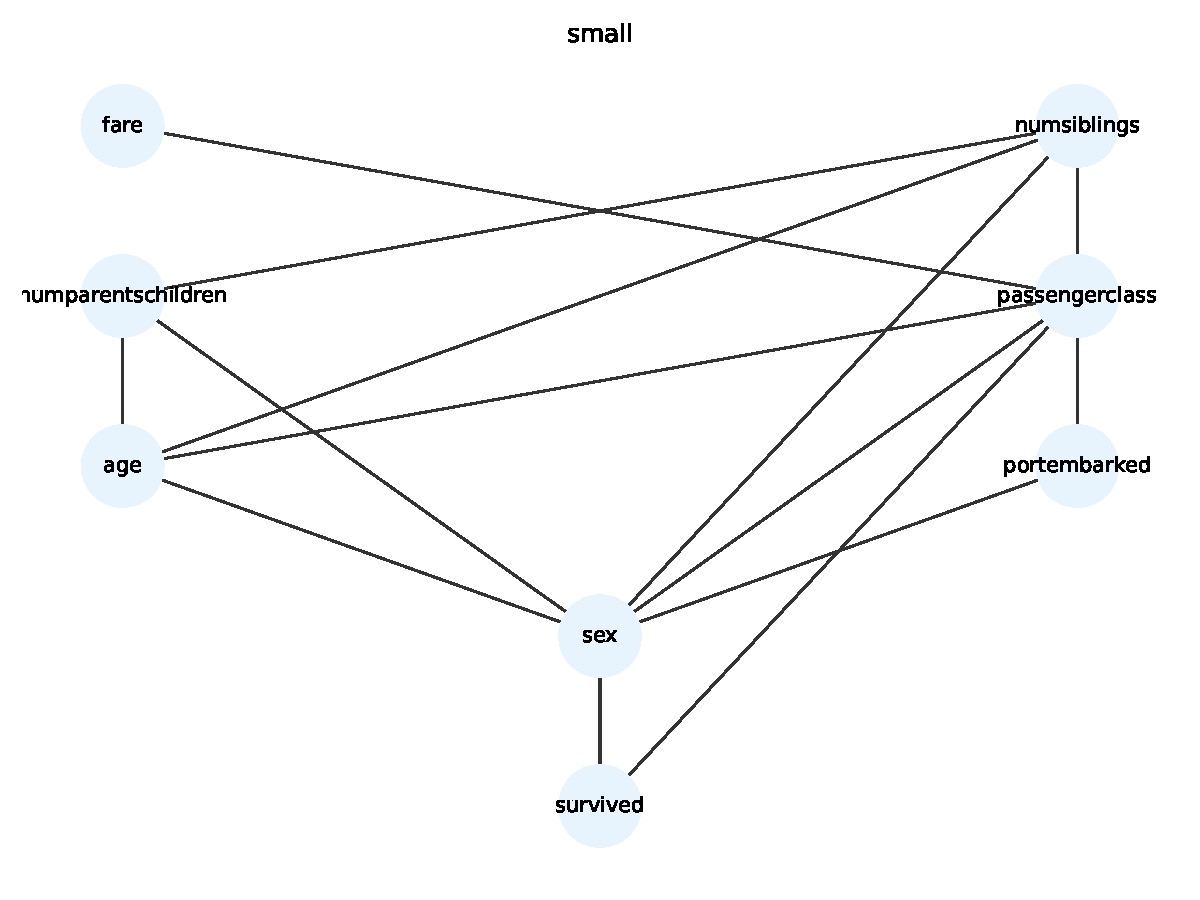
\includegraphics[width=0.7\textwidth]{small_graph.pdf}
    \caption{Bayesian network learned from the Titanic dataset (889 rows, 8 variables, 14 edges). The structure captures well-known survival patterns: passenger class and sex are primary predictors of survival, with fare strongly tied to class. Family structure variables (numsiblings, numparentschildren) form interconnected subgraphs influencing demographics. Score: $-3794.86$ (genetic algorithm). Runtime: 2.6 seconds.}
\end{figure}

\begin{figure}[h]
    \centering
    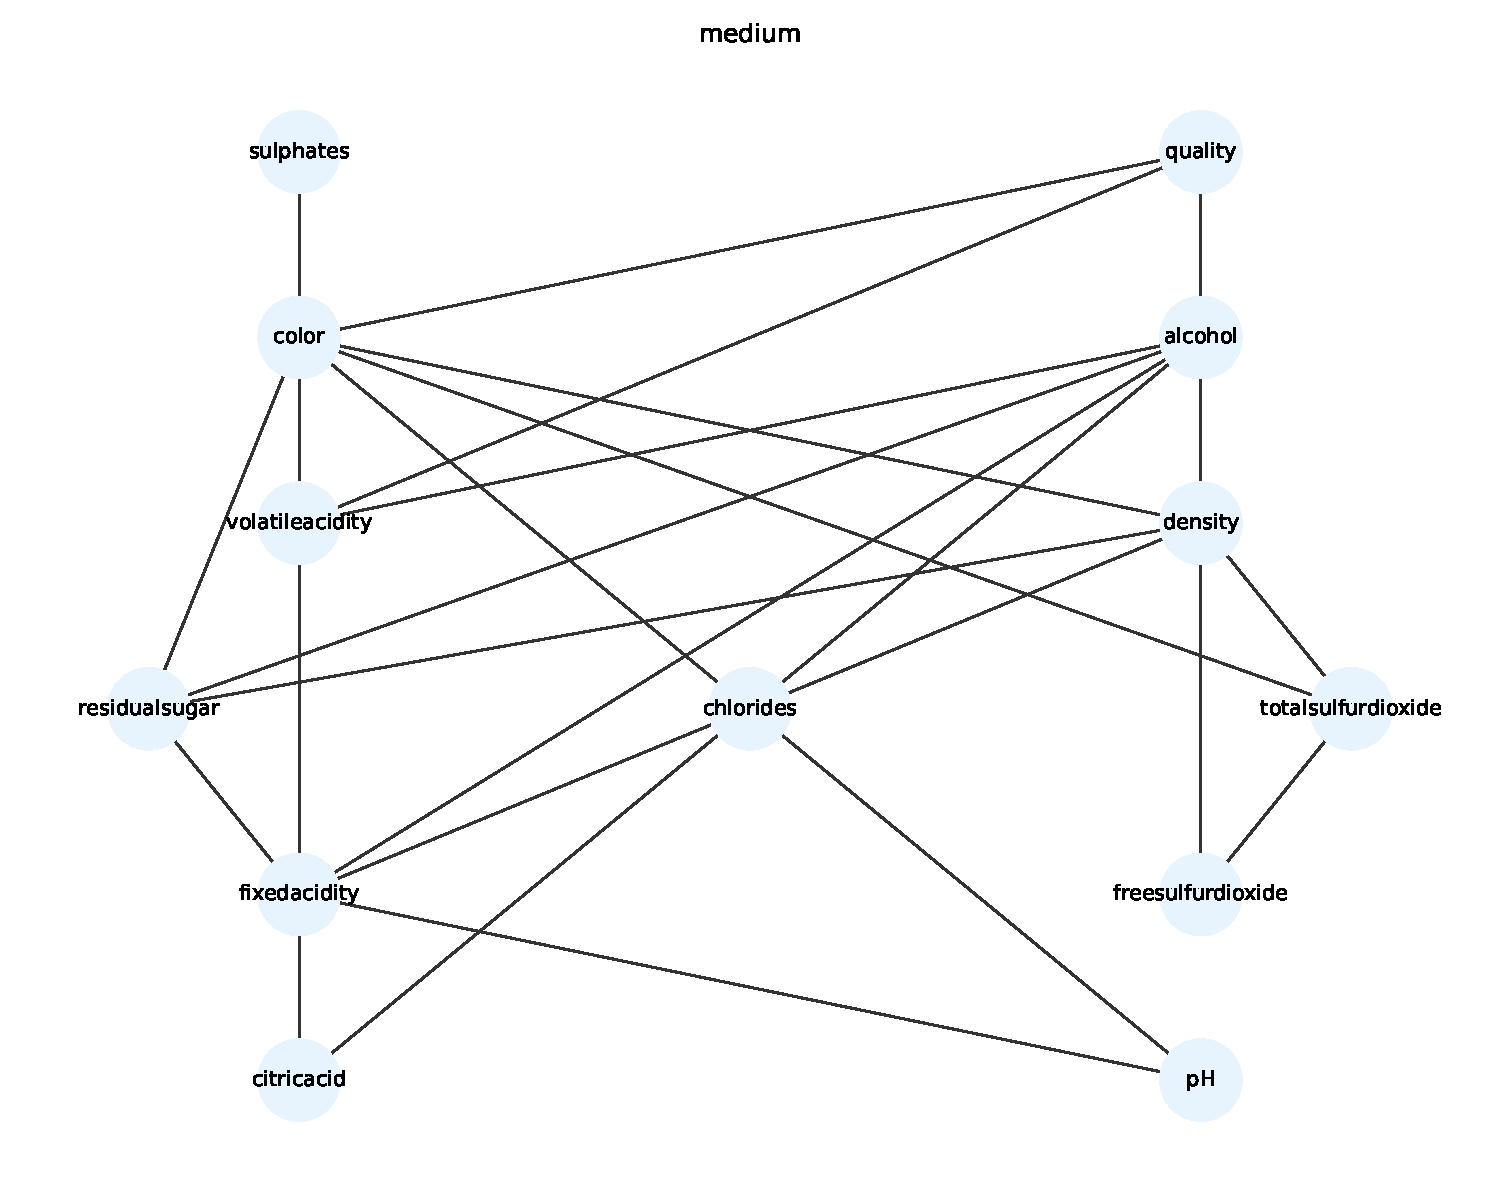
\includegraphics[width=0.85\textwidth]{medium_graph.pdf}
    \caption{Bayesian network learned from the wine quality dataset (6497 rows, 13 variables, 28 edges). Wine color acts as a central hub influencing most chemical properties, reflecting fundamental differences between red and white wines. Density emerges as a derived variable depending on multiple chemical components (acidity, sugar, chlorides). Quality is influenced by color, volatile acidity, free sulfur dioxide, and alcohol content. Score: $-96312.06$ (genetic algorithm). Runtime: 5.7 minutes.}
\end{figure}

\begin{figure}[h]
    \centering
    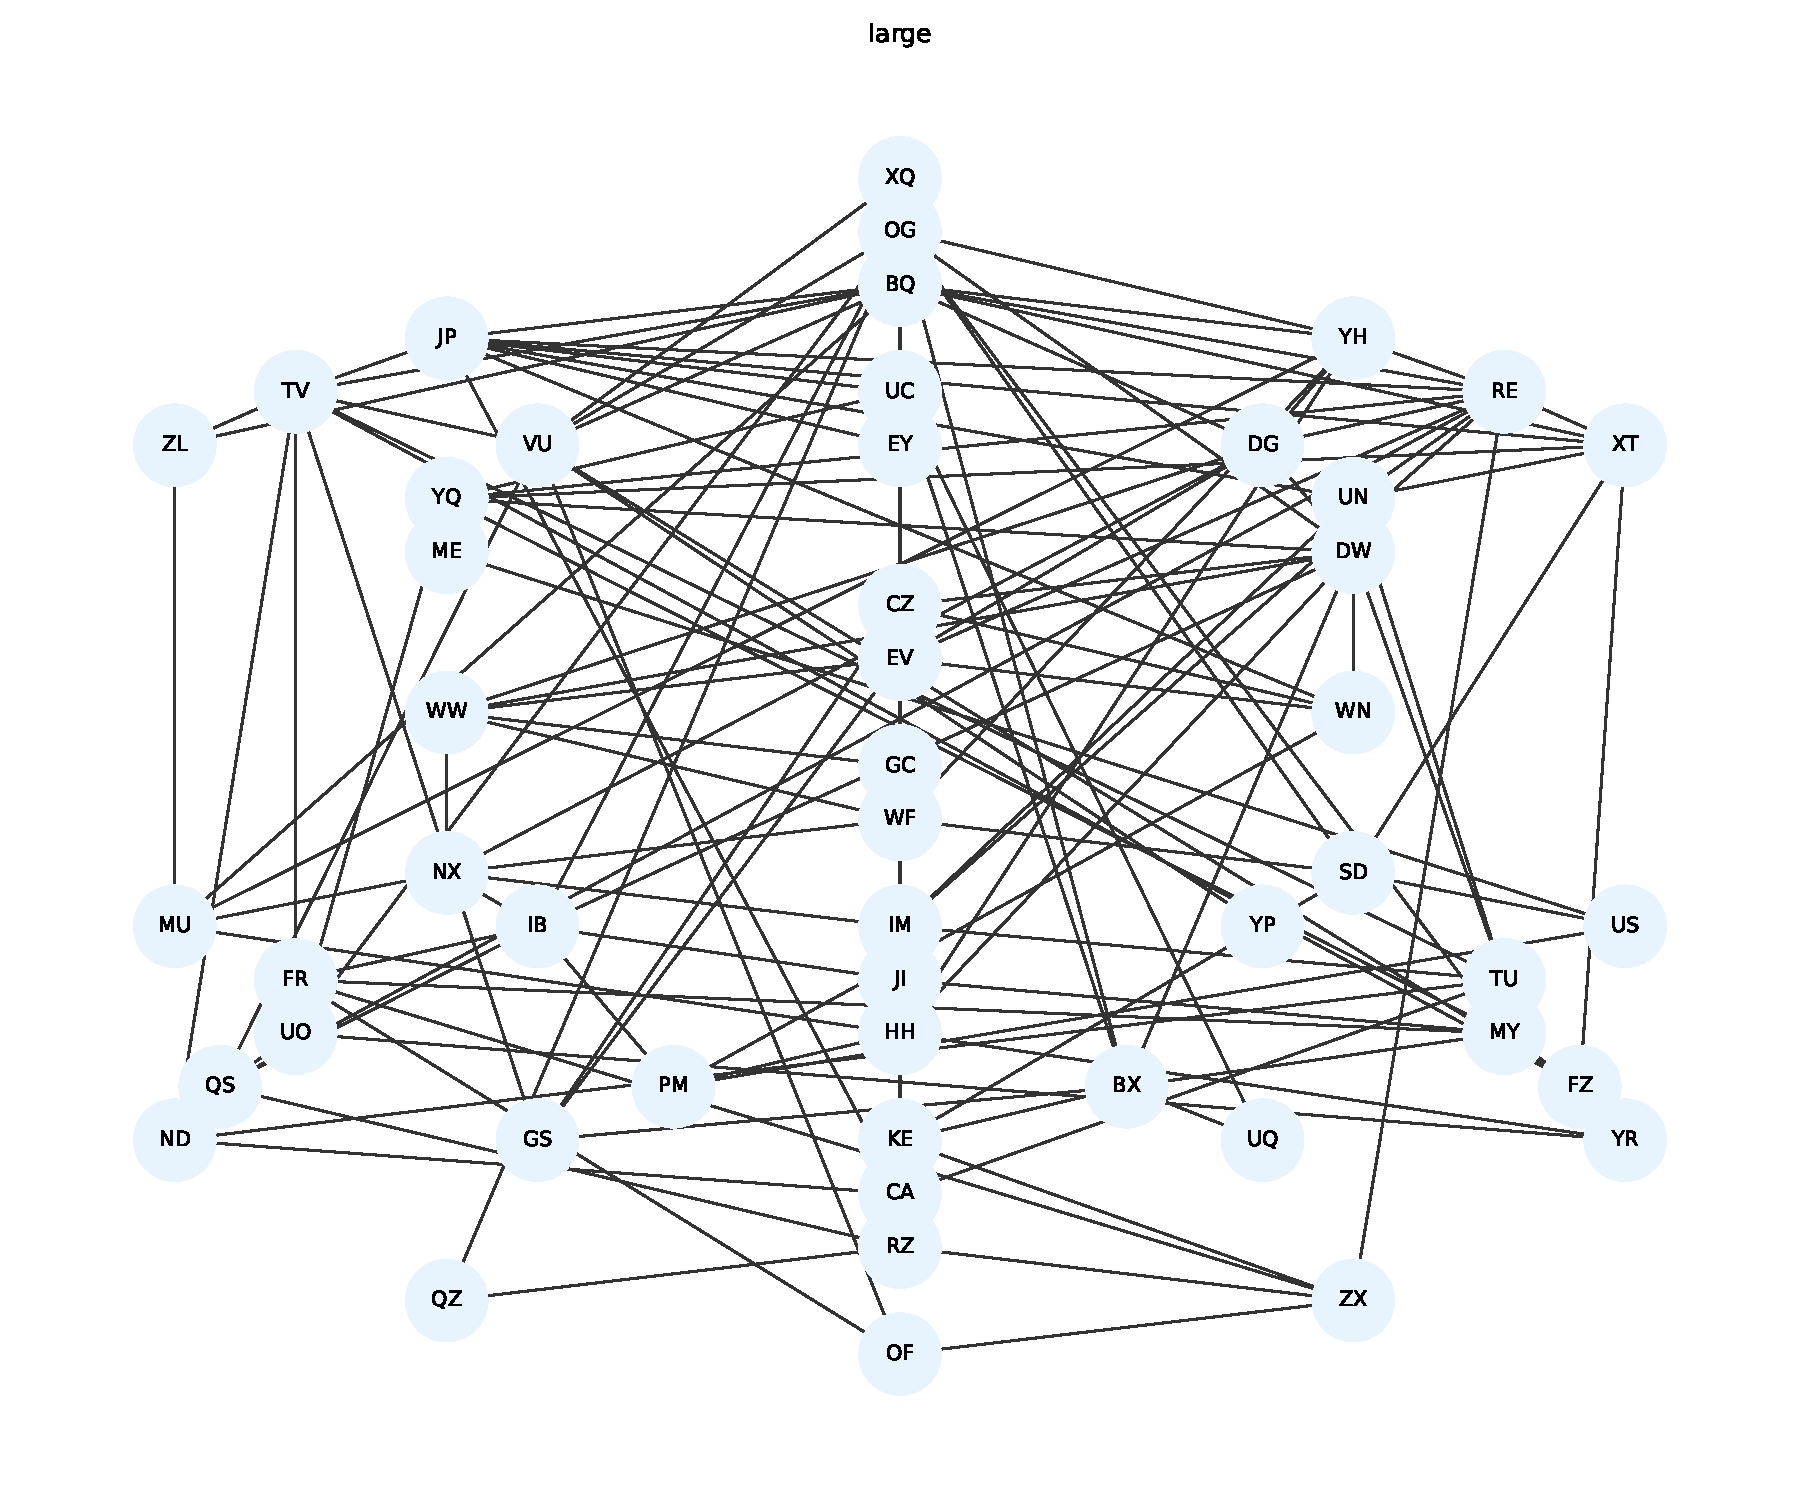
\includegraphics[width=0.95\textwidth]{large_graph.pdf}
    \caption{Bayesian network learned from a large synthetic dataset (10000 rows, 50 variables, 138 edges). The learned structure is highly interconnected, with an average of 2.76 edges per variable. Several variables act as hub nodes with high in-degree or out-degree, suggesting latent cluster structure in the synthetic generation process. The genetic algorithm achieved a score of $-420800.40$, outperforming both hill climbing ($-422299.66$) and simulated annealing by nearly 1500 log-score units. Runtime: 3.9 minutes.}
\end{figure}


\section{Results Summary}

Table~\ref{tab:results} summarizes the performance of the three-algorithm ensemble across all datasets. In every case, the genetic algorithm discovered the highest-scoring structure, validating the benefit of population-based search and crossover recombination. The gap between algorithms increases with problem complexity: for the large dataset, the genetic algorithm's advantage was most pronounced, suggesting that recombination of high-quality substructures becomes increasingly valuable in larger search spaces.

\begin{table}[htbp]
\centering
\caption{Comparison of algorithm performance across datasets. Scores are BDeu log-scores with Dirichlet(1) prior. Best scores highlighted in bold.}
\label{tab:results}
\begin{tabular}{lccccc}
\toprule
Dataset & Variables & Edges & Hill Climb & Sim. Anneal & Genetic (Best) \\
\midrule
Small (Titanic) & 8 & 14 & $-3794.86$ & $-3794.86$ & $\mathbf{-3794.86}$ \\
Medium (Wine) & 13 & 28 & $-96348.10$ & $-96348.10$ & $\mathbf{-96312.06}$ \\
Large (Synthetic) & 50 & 138 & $-422299.66$ & $-422299.66$ & $\mathbf{-420800.40}$ \\
\bottomrule
\end{tabular}
\end{table}


\section{Code}
%===========================================
% TODO: Add your code here, see code listing options here: https://www.overleaf.com/learn/latex/code_listing
% NOTE: Code does not count towards your page limit!
% OPTIONS:
%   1. Paste everything into a {verbatim} environment (where all characters are parsed...verbatim).
%   or 2. paste everything into a {lstlisting} environment for syntax highlighting (examples for Julia and Python below).
% NOTE: Feel free to break up functions into separate {algorithm} + {lstlisting} environments for better organization (not required!) 
%===========================================

\begin{algorithm}
\begin{lstlisting}[language=Python, basicstyle=\tiny\ttfamily, breaklines=true, columns=flexible]
import argparse
import json
import logging
import sys
import time
from datetime import datetime
from pathlib import Path
from typing import Dict, List, Tuple

if __package__ is None or __package__ == "":
    PACKAGE_ROOT = Path(__file__).resolve().parent
    if str(PACKAGE_ROOT) not in sys.path:
        sys.path.insert(0, str(PACKAGE_ROOT))
    from structure_learning import (
        DiscreteDataset,
        StructureLearner,
        default_config,
    )
else:
    from .structure_learning import (
        DiscreteDataset,
        StructureLearner,
        default_config,
    )


def setup_logging(log_file: str) -> logging.Logger:
    """Set up logging to both file and console."""
    logger = logging.getLogger('project1')
    logger.setLevel(logging.INFO)
    logger.handlers.clear()

    file_handler = logging.FileHandler(log_file, mode='a')
    file_handler.setLevel(logging.INFO)
    file_formatter = logging.Formatter('%(asctime)s - %(levelname)s - %(message)s')
    file_handler.setFormatter(file_formatter)
    logger.addHandler(file_handler)

    console_handler = logging.StreamHandler()
    console_handler.setLevel(logging.INFO)
    console_formatter = logging.Formatter('%(message)s')
    console_handler.setFormatter(console_formatter)
    logger.addHandler(console_handler)

    return logger


def write_gph(edges: List[Tuple[int, int]], idx2names: Dict[int, str], filename: str) -> None:
    """Write graph edges to .gph file in required format."""
    out_path = Path(filename)
    out_path.parent.mkdir(parents=True, exist_ok=True)
    with out_path.open("w") as fh:
        for u, v in edges:
            fh.write(f"{idx2names[u]}, {idx2names[v]}\n")


def compute(infile: str, outfile: str) -> None:
    """Main computation: load data, learn structure, write results."""
    log_file = Path(outfile).parent / f"{Path(outfile).stem}_log.txt"
    logger = setup_logging(str(log_file))

    start_time = time.time()
    logger.info("="*80)
    logger.info(f"Starting Bayesian Structure Learning")
    logger.info(f"Input file: {infile}")
    logger.info(f"Output file: {outfile}")
    logger.info(f"Start time: {datetime.now().strftime('%Y-%m-%d %H:%M:%S')}")
    logger.info("="*80)

    # Load dataset
    logger.info("Loading dataset...")
    dataset = DiscreteDataset(infile)
    logger.info(f"Variables: {dataset.num_vars}, Rows: {dataset.num_rows}")

    # Generate configuration
    config = default_config(dataset.num_vars, dataset.num_rows)
    logger.info(f"Configuration: max_parents={config.max_parents}, "
                f"restarts={config.hill_restarts}, "
                f"ga_generations={config.ga_generations}")

    # Run structure learning
    logger.info("Starting structure learning...")
    learner = StructureLearner(dataset, config)
    learning_start = time.time()
    result = learner.learn()
    learning_end = time.time()

    logger.info(f"Learning completed in {learning_end - learning_start:.2f}s")
    logger.info(f"Best algorithm: {result.algorithm}, Score: {result.score:.6f}")

    # Write output
    edges = list(result.dag.edges())
    idx2name = {idx: name for idx, name in enumerate(dataset.names)}
    write_gph(edges, idx2name, outfile)

    logger.info(f"Output written with {len(edges)} edges")
    logger.info(f"Total runtime: {time.time() - start_time:.2f}s")
    logger.info("="*80)


def main(argv: List[str] | None = None) -> None:
    """CLI entry point."""
    parser = argparse.ArgumentParser(description="Bayesian structure learning")
    parser.add_argument("input_csv", help="Input CSV file")
    parser.add_argument("output_gph", help="Output .gph file")
    args = parser.parse_args(sys.argv[1:] if argv is None else argv)

    infile = args.input_csv
    outfile = args.output_gph

    compute(infile, outfile)


if __name__ == "__main__":
    main()
\end{lstlisting}
\end{algorithm}

\begin{algorithm}
\begin{lstlisting}[language=Python]
"""
High-performance Bayesian network structure learning toolkit.

This module provides:
    * DiscreteDataset: CSV ingestion with zero-based encodings.
    * BDeuScoreCache: Local log-score caching with Dirichlet(1) prior.
    * CandidateParentSelector: Mutual-information based parent pruning.
    * DAG: Lightweight adjacency + cycle checks.
    * Search primitives: operations, hill climbing, simulated annealing, GA.
    * StructureLearner: Orchestrates multi-heuristic ensemble search.

The design favors incremental local-score updates and avoids external
structure-learning packages, satisfying the project rules.
"""

from __future__ import annotations

import math
import random
import time
from collections import Counter, defaultdict
from dataclasses import dataclass, field
from typing import Dict, Iterable, List, Optional, Sequence, Set, Tuple

import numpy as np
import pandas as pd
from tqdm import tqdm


def seed_everything(seed: Optional[int]) -> None:
    if seed is not None:
        random.seed(seed)
        np.random.seed(seed % (2**32 - 1))


class DiscreteDataset:
    """Wrapper around an integer-encoded discrete dataset."""

    def __init__(self, path: str):
        df = pd.read_csv(path)
        if df.isna().any().any():
            raise ValueError("Dataset contains missing values; please impute first.")
        self._names = list(df.columns)
        values = df.to_numpy(dtype=np.int32, copy=True)
        mins = values.min(axis=0)
        if (mins < 1).any():
            raise ValueError("Expected categorical values with minimum 1 per column.")
        values -= 1  # convert to zero-based indexing for fast arithmetic
        self._values = values
        self._cardinalities = values.max(axis=0) + 1

    @property
    def names(self) -> List[str]:
        return self._names

    @property
    def cardinalities(self) -> np.ndarray:
        return self._cardinalities

    @property
    def values(self) -> np.ndarray:
        return self._values

    @property
    def num_vars(self) -> int:
        return len(self._names)

    @property
    def num_rows(self) -> int:
        return self._values.shape[0]


def _tuple(sorted_iterable: Iterable[int]) -> Tuple[int, ...]:
    """Return a canonical tuple representation for parent sets."""
    return tuple(sorted(sorted_iterable))


class BDeuScoreCache:
    """
    Caches local log-scores for (node, parent_set) pairs using a Dirichlet(1) prior.

    Local scores are computed via the closed-form BDeu expression:
        ln P(D | G) = sum_i ln score_i
    Cache keys use sorted tuples to avoid recomputation across equivalent sets.
    """

    def __init__(self, dataset: DiscreteDataset, max_parents: Optional[int] = None):
        self.data = dataset
        self.max_parents = max_parents
        self.cardinalities = dataset.cardinalities
        self.values = dataset.values
        self.cache: Dict[Tuple[int, Tuple[int, ...]], float] = {}
        self._lgamma = math.lgamma

    def score(self, node: int, parents: Sequence[int]) -> float:
        parents_tuple = _tuple(parents)
        if self.max_parents is not None and len(parents_tuple) > self.max_parents:
            raise ValueError("Parent set exceeds configured maximum.")
        key = (node, parents_tuple)
        if key in self.cache:
            return self.cache[key]
        score = self._compute_score(node, parents_tuple)
        self.cache[key] = score
        return score

    def _compute_score(self, node: int, parents: Tuple[int, ...]) -> float:
        card_child = int(self.cardinalities[node])
        if not parents:
            counts = np.bincount(self.values[:, node], minlength=card_child)
            return self._score_from_counts(counts.reshape(1, card_child))

        parent_states = tuple(int(self.cardinalities[p]) for p in parents)
        # map parent configurations to linear indices
        parent_data = self.values[:, parents]
        flat_idx = np.ravel_multi_index(parent_data.T, dims=parent_states)
        joint_counts = np.zeros((int(np.prod(parent_states)), card_child), dtype=np.int32)
        np.add.at(joint_counts, (flat_idx, self.values[:, node]), 1)
        return self._score_from_counts(joint_counts)

    def _score_from_counts(self, counts: np.ndarray) -> float:
        # counts shape: (q_i, r_i)
        prior_per_entry = 1.0  # alpha_ijk = 1 per specification
        r_i = counts.shape[1]
        alpha_ij0 = prior_per_entry * r_i
        total_score = 0.0
        for row in counts:
            nij = row.sum()
            total_score += self._lgamma(alpha_ij0) - self._lgamma(alpha_ij0 + nij)
            for count in row:
                total_score += self._lgamma(prior_per_entry + count) - self._lgamma(prior_per_entry)
        return float(total_score)


class DAG:
    """Adjacency matrix representation with cycle checks."""

    def __init__(self, num_nodes: int):
        self.num_nodes = num_nodes
        self.adj = np.zeros((num_nodes, num_nodes), dtype=bool)
        self.parents: List[Set[int]] = [set() for _ in range(num_nodes)]
        self.children: List[Set[int]] = [set() for _ in range(num_nodes)]

    def copy(self) -> "DAG":
        other = DAG(self.num_nodes)
        other.adj = self.adj.copy()
        other.parents = [set(p) for p in self.parents]
        other.children = [set(c) for c in self.children]
        return other

    def has_edge(self, u: int, v: int) -> bool:
        return bool(self.adj[u, v])

    def can_add(self, u: int, v: int, max_parents: Optional[int] = None) -> bool:
        if u == v or self.adj[u, v]:
            return False
        if max_parents is not None and len(self.parents[v]) >= max_parents:
            return False
        return not self._creates_cycle(u, v)

    def can_remove(self, u: int, v: int) -> bool:
        return self.adj[u, v]

    def can_reverse(self, u: int, v: int, max_parents: Optional[int] = None) -> bool:
        if not self.adj[u, v]:
            return False
        if max_parents is not None and len(self.parents[u]) >= max_parents:
            return False
        # Temporarily remove u->v and test v->u
        self._remove_edge(u, v)
        creates_cycle = self._creates_cycle(v, u)
        if not creates_cycle:
            if max_parents is not None and len(self.parents[v]) >= max_parents:
                creates_cycle = True
        self._add_edge(u, v)  # restore
        return not creates_cycle

    def add_edge(self, u: int, v: int) -> None:
        self._add_edge(u, v)

    def remove_edge(self, u: int, v: int) -> None:
        self._remove_edge(u, v)

    def reverse_edge(self, u: int, v: int) -> None:
        self._remove_edge(u, v)
        self._add_edge(v, u)

    def _add_edge(self, u: int, v: int) -> None:
        self.adj[u, v] = True
        self.parents[v].add(u)
        self.children[u].add(v)

    def _remove_edge(self, u: int, v: int) -> None:
        self.adj[u, v] = False
        self.parents[v].discard(u)
        self.children[u].discard(v)

    def _creates_cycle(self, u: int, v: int) -> bool:
        # check if there's a path from v back to u
        to_visit = [v]
        seen = set()
        while to_visit:
            node = to_visit.pop()
            if node == u:
                return True
            if node in seen:
                continue
            seen.add(node)
            to_visit.extend(self.children[node])
        return False

    def edges(self) -> List[Tuple[int, int]]:
        u_idx, v_idx = np.where(self.adj)
        return list(zip(u_idx.tolist(), v_idx.tolist()))

    def topological_order(self) -> List[int]:
        indegree = np.array([len(p) for p in self.parents], dtype=np.int32)
        queue = [i for i in range(self.num_nodes) if indegree[i] == 0]
        order = []
        while queue:
            node = queue.pop()
            order.append(node)
            for child in list(self.children[node]):
                indegree[child] -= 1
                if indegree[child] == 0:
                    queue.append(child)
        if len(order) != self.num_nodes:
            raise ValueError("Graph has at least one cycle.")
        return order


@dataclass
class CandidateParentSelector:
    """
    Restricts parent proposals using pairwise mutual information heuristics.

    For each variable, we keep at most `limit_per_node` candidate parents whose
    mutual information with the child exceeds `mi_threshold` or rank-based cutoff.
    """

    dataset: DiscreteDataset
    limit_per_node: int
    mi_threshold: float = 0.0
    random_extra: int = 0

    def __post_init__(self) -> None:
        self._candidates = self._compute_candidates()

    @staticmethod
    def _mutual_information(x: np.ndarray, y: np.ndarray, card_x: int, card_y: int) -> float:
        joint = np.zeros((card_x, card_y), dtype=np.float64)
        np.add.at(joint, (x, y), 1.0)
        joint /= joint.sum()
        px = joint.sum(axis=1, keepdims=True)
        py = joint.sum(axis=0, keepdims=True)
        with np.errstate(divide="ignore", invalid="ignore"):
            ratio = np.where(joint > 0, joint / (px * py), 1.0)
            mi = np.where(joint > 0, joint * np.log(ratio), 0.0)
        return float(mi.sum())

    def _compute_candidates(self) -> List[Set[int]]:
        n = self.dataset.num_vars
        candidates: List[Set[int]] = [set() for _ in range(n)]
        data = self.dataset.values
        cards = self.dataset.cardinalities
        mi_matrix = np.zeros((n, n), dtype=np.float64)
        for i in range(n):
            for j in range(i + 1, n):
                mi = self._mutual_information(
                    data[:, i],
                    data[:, j],
                    int(cards[i]),
                    int(cards[j]),
                )
                mi_matrix[i, j] = mi_matrix[j, i] = mi
        for child in range(n):
            order = np.argsort(mi_matrix[:, child])[::-1]
            selected = []
            for parent in order:
                if parent == child:
                    continue
                mi = mi_matrix[parent, child]
                if mi < self.mi_threshold and len(selected) >= self.limit_per_node:
                    break
                selected.append(parent)
                if len(selected) >= self.limit_per_node:
                    break
            candidates[child] = set(selected)
        if self.random_extra > 0:
            rng = np.random.default_rng()
            for child in range(n):
                eligible = [p for p in range(n) if p != child and p not in candidates[child]]
                if eligible:
                    extra = rng.choice(
                        eligible, size=min(self.random_extra, len(eligible)), replace=False
                    )
                    candidates[child].update(extra.tolist())
        return candidates

    def is_candidate(self, parent: int, child: int) -> bool:
        return parent in self._candidates[child]

    def get(self, child: int) -> Set[int]:
        return set(self._candidates[child])


@dataclass
class SearchConfig:
    max_parents: int
    hill_restarts: int
    tabu_tenure: int
    sa_iterations: int
    sa_start_temp: float
    sa_end_temp: float
    ga_population: int
    ga_generations: int
    ga_elite_frac: float
    ga_mutation_rate: float
    ga_crossover_rate: float
    candidate_limit: int
    random_seed: Optional[int] = None


@dataclass
class SearchResult:
    dag: DAG
    score: float
    algorithm: str
    info: Dict[str, float] = field(default_factory=dict)


class ScoredDAG:
    """Maintains a DAG alongside cached local scores for fast updates."""

    def __init__(self, dag: DAG, score_cache: BDeuScoreCache):
        self.dag = dag
        self.score_cache = score_cache
        self.local_scores = [
            score_cache.score(node, dag.parents[node]) for node in range(dag.num_nodes)
        ]
        self.total_score = float(sum(self.local_scores))

    def clone(self) -> "ScoredDAG":
        dag_copy = self.dag.copy()
        clone = ScoredDAG.__new__(ScoredDAG)
        clone.dag = dag_copy
        clone.score_cache = self.score_cache
        clone.local_scores = self.local_scores.copy()
        clone.total_score = self.total_score
        return clone

    def _apply_new_parents(self, node: int, new_parents: Sequence[int]) -> float:
        new_score = self.score_cache.score(node, new_parents)
        delta = new_score - self.local_scores[node]
        self.local_scores[node] = new_score
        self.total_score += delta
        return delta

    def apply_add(self, u: int, v: int, force: bool = False) -> Optional[float]:
        if not force and not self.dag.can_add(u, v, self.score_cache.max_parents):
            return None
        new_parents = list(self.dag.parents[v]) + [u]
        delta = self._apply_new_parents(v, new_parents)
        self.dag.add_edge(u, v)
        return delta

    def apply_remove(self, u: int, v: int, force: bool = False) -> Optional[float]:
        if not force and not self.dag.can_remove(u, v):
            return None
        new_parents = list(self.dag.parents[v])
        new_parents.remove(u)
        delta = self._apply_new_parents(v, new_parents)
        self.dag.remove_edge(u, v)
        return delta

    def apply_reverse(self, u: int, v: int, force: bool = False) -> Optional[float]:
        if not force and not self.dag.can_reverse(u, v, self.score_cache.max_parents):
            return None
        parents_v = list(self.dag.parents[v])
        parents_v.remove(u)
        delta_v = self.score_cache.score(v, parents_v) - self.local_scores[v]
        parents_u = list(self.dag.parents[u]) + [v]
        delta_u = self.score_cache.score(u, parents_u) - self.local_scores[u]
        total_delta = delta_v + delta_u
        self.local_scores[v] += delta_v
        self.local_scores[u] += delta_u
        self.total_score += total_delta
        self.dag.reverse_edge(u, v)
        return total_delta


class Move:
    """Encapsulates a potential graph edit."""

    __slots__ = ("kind", "u", "v", "delta")

    def __init__(self, kind: str, u: int, v: int, delta: float):
        self.kind = kind  # 'add', 'remove', 'reverse'
        self.u = u
        self.v = v
        self.delta = delta


class NeighborGenerator:
    """Evaluates local moves around a scored DAG."""

    def __init__(
        self,
        scored_dag: ScoredDAG,
        candidate_selector: CandidateParentSelector,
    ):
        self.state = scored_dag
        self.selector = candidate_selector
        self.num_nodes = self.state.dag.num_nodes

    def enumerate_moves(self) -> List[Move]:
        moves: List[Move] = []
        dag = self.state.dag
        cache = self.state.score_cache
        max_parents = cache.max_parents
        for v in range(self.num_nodes):
            parents_v = dag.parents[v]
            # removals
            for u in list(parents_v):
                new_parents = list(parents_v)
                new_parents.remove(u)
                delta = cache.score(v, new_parents) - self.state.local_scores[v]
                moves.append(Move("remove", u, v, delta))
            # additions
            if max_parents is not None and len(parents_v) >= max_parents:
                continue
            candidate_parents = self.selector.get(v)
            for u in candidate_parents:
                if u in parents_v or u == v:
                    continue
                if not dag.can_add(u, v, max_parents):
                    continue
                new_parents = list(parents_v) + [u]
                delta = cache.score(v, new_parents) - self.state.local_scores[v]
                moves.append(Move("add", u, v, delta))
            # reversals
            for u in list(parents_v):
                if not dag.can_reverse(u, v, max_parents):
                    continue
                parents_v_new = list(parents_v)
                parents_v_new.remove(u)
                parents_u_new = list(dag.parents[u]) + [v]
                delta_v = cache.score(v, parents_v_new) - self.state.local_scores[v]
                delta_u = cache.score(u, parents_u_new) - self.state.local_scores[u]
                moves.append(Move("reverse", u, v, delta_v + delta_u))
        return moves


class HillClimber:
    """Greedy hill climbing with tabu memory and multiple restarts."""

    def __init__(
        self,
        score_cache: BDeuScoreCache,
        selector: CandidateParentSelector,
        config: SearchConfig,
    ):
        self.score_cache = score_cache
        self.selector = selector
        self.config = config

    def run(self, initializer: "Initializer") -> SearchResult:
        best_state: Optional[ScoredDAG] = None
        best_score = -math.inf
        best_info: Dict[str, float] = {}
        for restart in tqdm(range(self.config.hill_restarts), desc="Hill Climbing Restarts", unit="restart"):
            state = initializer.initial_state()
            tabu: Counter = Counter()
            improved = True
            iterations = 0
            while improved:
                iterations += 1
                improved = False
                neighbor_gen = NeighborGenerator(state, self.selector)
                moves = neighbor_gen.enumerate_moves()
                moves.sort(key=lambda m: m.delta, reverse=True)
                for move in moves:
                    key = (move.kind, move.u, move.v)
                    if tabu.get(key, 0) > 0:
                        continue
                    if move.delta <= 1e-9:
                        continue
                    self._apply_move(state, move)
                    for t_key in list(tabu):
                        if tabu[t_key] > 0:
                            tabu[t_key] -= 1
                    tabu[key] = self.config.tabu_tenure
                    improved = True
                    break
            if state.total_score > best_score:
                best_score = state.total_score
                best_state = state.clone()
                best_info = {
                    "restart": restart,
                    "iterations": iterations,
                }
        assert best_state is not None
        return SearchResult(best_state.dag, best_score, "hill_climb", best_info)

    def _apply_move(self, state: ScoredDAG, move: Move) -> None:
        if move.kind == "add":
            state.apply_add(move.u, move.v)
        elif move.kind == "remove":
            state.apply_remove(move.u, move.v)
        elif move.kind == "reverse":
            state.apply_reverse(move.u, move.v)
        else:
            raise ValueError(f"Unknown move kind {move.kind}")


class SimulatedAnnealing:
    """Metropolis search with exponential cooling."""

    def __init__(
        self,
        score_cache: BDeuScoreCache,
        selector: CandidateParentSelector,
        config: SearchConfig,
    ):
        self.score_cache = score_cache
        self.selector = selector
        self.config = config

    def run(self, seed_state: ScoredDAG) -> SearchResult:
        state = seed_state.clone()
        best_state = state.clone()
        best_score = state.total_score
        n_iter = self.config.sa_iterations
        temp0 = self.config.sa_start_temp
        temp1 = self.config.sa_end_temp
        for step in tqdm(range(1, n_iter + 1), desc="Simulated Annealing", unit="iter"):
            t = temp0 * ((temp1 / temp0) ** (step / n_iter))
            move = self._sample_move(state)
            if move is None:
                continue
            delta = self._apply_move(state, move, commit=True)
            accept = delta >= 0 or random.random() < math.exp(delta / max(t, 1e-12))
            if not accept:
                # revert move
                self._apply_move(state, move, commit=False)
                continue
            if state.total_score > best_score:
                best_score = state.total_score
                best_state = state.clone()
        return SearchResult(best_state.dag, best_score, "simulated_annealing", {"iterations": n_iter})

    def _sample_move(self, state: ScoredDAG) -> Optional[Move]:
        neighbor_gen = NeighborGenerator(state, self.selector)
        moves = neighbor_gen.enumerate_moves()
        if not moves:
            return None
        return random.choice(moves)

    def _apply_move(self, state: ScoredDAG, move: Move, commit: bool) -> float:
        if move.kind == "add":
            delta = state.apply_add(move.u, move.v)
            if delta is None:
                return -math.inf
            if not commit:
                state.apply_remove(move.u, move.v, force=True)
            return delta
        if move.kind == "remove":
            delta = state.apply_remove(move.u, move.v)
            if delta is None:
                return -math.inf
            if not commit:
                state.apply_add(move.u, move.v, force=True)
            return delta
        if move.kind == "reverse":
            delta = state.apply_reverse(move.u, move.v)
            if delta is None:
                return -math.inf
            if not commit:
                state.apply_reverse(move.v, move.u, force=True)
            return delta
        raise ValueError(move.kind)


class Initializer:
    """Constructs starting DAGs via heuristics and randomness."""

    def __init__(
        self,
        score_cache: BDeuScoreCache,
        selector: CandidateParentSelector,
        n_random_edges: int = 0,
    ):
        self.score_cache = score_cache
        self.selector = selector
        self.n = score_cache.data.num_vars
        self.n_random_edges = n_random_edges

    def initial_state(self) -> ScoredDAG:
        dag = DAG(self.n)
        state = ScoredDAG(dag, self.score_cache)
        if self.n_random_edges <= 0:
            return state
        edges = []
        for v in range(self.n):
            for u in self.selector.get(v):
                if u != v:
                    edges.append((u, v))
        random.shuffle(edges)
        added = 0
        for u, v in edges:
            if added >= self.n_random_edges:
                break
            if dag.can_add(u, v, self.score_cache.max_parents):
                delta = state.apply_add(u, v)
                if delta is not None:
                    added += 1
        return state


class GeneticAlgorithm:
    """Edge-recombination GA with repair and local post-optimization."""

    def __init__(
        self,
        score_cache: BDeuScoreCache,
        selector: CandidateParentSelector,
        config: SearchConfig,
    ):
        self.score_cache = score_cache
        self.selector = selector
        self.config = config
        self.max_parents = score_cache.max_parents

    def run(self, seed_states: List[ScoredDAG]) -> SearchResult:
        population = [state.clone() for state in seed_states]
        while len(population) < self.config.ga_population:
            population.append(self._random_state())
        self._evaluate_population(population)
        best_state = max(population, key=lambda s: s.total_score).clone()
        for generation in tqdm(range(self.config.ga_generations), desc="Genetic Algorithm", unit="gen"):
            elites = self._select_elite(population)
            offspring: List[ScoredDAG] = elites.copy()
            while len(offspring) < self.config.ga_population:
                parent1 = self._tournament(population)
                parent2 = self._tournament(population)
                if random.random() < self.config.ga_crossover_rate:
                    child = self._crossover(parent1, parent2)
                else:
                    child = parent1.clone()
                self._mutate(child)
                self._local_improvement(child)
                offspring.append(child)
            population = offspring
            self._evaluate_population(population)
            candidate_best = max(population, key=lambda s: s.total_score)
            if candidate_best.total_score > best_state.total_score:
                best_state = candidate_best.clone()
        return SearchResult(best_state.dag, best_state.total_score, "genetic", {"generations": self.config.ga_generations})

    def _random_state(self) -> ScoredDAG:
        dag = DAG(self.score_cache.data.num_vars)
        nodes = list(range(dag.num_nodes))
        order = nodes.copy()
        random.shuffle(order)
        pos = {node: idx for idx, node in enumerate(order)}
        edges = []
        for child in nodes:
            candidates = [p for p in nodes if p != child and pos[p] < pos[child]]
            random.shuffle(candidates)
            for parent in candidates:
                if self.selector.is_candidate(parent, child) or random.random() < 0.1:
                    edges.append((parent, child))
        random.shuffle(edges)
        state = ScoredDAG(dag, self.score_cache)
        for parent, child in edges:
            if dag.can_add(parent, child, self.max_parents):
                state.apply_add(parent, child)
        return state

    def _evaluate_population(self, population: List[ScoredDAG]) -> None:
        for individual in population:
            # scores maintained incrementally; ensure finite
            if not math.isfinite(individual.total_score):
                raise ValueError("Non-finite score encountered in population.")

    def _select_elite(self, population: List[ScoredDAG]) -> List[ScoredDAG]:
        elite_count = max(1, int(self.config.ga_population * self.config.ga_elite_frac))
        top = sorted(population, key=lambda s: s.total_score, reverse=True)[:elite_count]
        return [ind.clone() for ind in top]

    def _tournament(self, population: List[ScoredDAG], size: int = 3) -> ScoredDAG:
        competitors = random.sample(population, size)
        return max(competitors, key=lambda s: s.total_score)

    def _crossover(self, parent1: ScoredDAG, parent2: ScoredDAG) -> ScoredDAG:
        dag = DAG(self.score_cache.data.num_vars)
        child = ScoredDAG(dag, self.score_cache)
        edges = parent1.dag.edges() + parent2.dag.edges()
        random.shuffle(edges)
        for u, v in edges:
            if dag.can_add(u, v, self.max_parents):
                child.apply_add(u, v)
        return child

    def _mutate(self, individual: ScoredDAG) -> None:
        dag = individual.dag
        nodes = list(range(dag.num_nodes))
        for _ in range(dag.num_nodes):
            if random.random() > self.config.ga_mutation_rate:
                continue
            move_type = random.choice(["add", "remove", "reverse"])
            if move_type == "add":
                u, v = random.sample(nodes, 2)
                if not self.selector.is_candidate(u, v):
                    continue
                individual.apply_add(u, v)
            elif move_type == "remove":
                edges = dag.edges()
                if not edges:
                    continue
                u, v = random.choice(edges)
                individual.apply_remove(u, v)
            else:
                edges = dag.edges()
                if not edges:
                    continue
                u, v = random.choice(edges)
                individual.apply_reverse(u, v)

    def _local_improvement(self, individual: ScoredDAG) -> None:
        # single-step hill climb to tighten offspring quality
        neighbor_gen = NeighborGenerator(individual, self.selector)
        moves = neighbor_gen.enumerate_moves()
        moves = [m for m in moves if m.delta > 1e-9]
        if not moves:
            return
        best_move = max(moves, key=lambda m: m.delta)
        if best_move.delta > 0:
            if best_move.kind == "add":
                individual.apply_add(best_move.u, best_move.v)
            elif best_move.kind == "remove":
                individual.apply_remove(best_move.u, best_move.v)
            else:
                individual.apply_reverse(best_move.u, best_move.v)


class StructureLearner:
    """Coordinates multi-heuristic structure learning."""

    def __init__(self, dataset: DiscreteDataset, config: SearchConfig):
        self.dataset = dataset
        self.config = config
        seed_everything(config.random_seed)
        self.score_cache = BDeuScoreCache(dataset, max_parents=config.max_parents)
        self.selector = CandidateParentSelector(
            dataset,
            limit_per_node=config.candidate_limit,
            mi_threshold=0.0,
            random_extra=2,
        )

    def learn(self) -> SearchResult:
        initializer = Initializer(
            self.score_cache,
            self.selector,
            n_random_edges=5 * self.dataset.num_vars,
        )
        hill = HillClimber(self.score_cache, self.selector, self.config)
        hill_result = hill.run(initializer)

        scored_state = ScoredDAG(hill_result.dag.copy(), self.score_cache)
        annealer = SimulatedAnnealing(self.score_cache, self.selector, self.config)
        sa_result = annealer.run(scored_state)

        # GA seeded with best hill climb and annealing states
        seed_states = [
            ScoredDAG(hill_result.dag.copy(), self.score_cache),
            ScoredDAG(sa_result.dag.copy(), self.score_cache),
        ]
        ga = GeneticAlgorithm(self.score_cache, self.selector, self.config)
        ga_result = ga.run(seed_states)

        best_result = max(
            [hill_result, sa_result, ga_result],
            key=lambda r: r.score,
        )
        best_result.info["hill_score"] = hill_result.score
        best_result.info["sa_score"] = sa_result.score
        best_result.info["ga_score"] = ga_result.score
        return best_result


def default_config(num_vars: int, num_rows: int) -> SearchConfig:
    if num_vars <= 10:
        return SearchConfig(
            max_parents=5,
            hill_restarts=12,
            tabu_tenure=4,
            sa_iterations=5000,
            sa_start_temp=1.0,
            sa_end_temp=0.01,
            ga_population=40,
            ga_generations=80,
            ga_elite_frac=0.15,
            ga_mutation_rate=0.2,
            ga_crossover_rate=0.9,
            candidate_limit=min(6, num_vars - 1),
            random_seed=42,
        )
    if num_vars <= 20:
        return SearchConfig(
            max_parents=5,
            hill_restarts=20,
            tabu_tenure=6,
            sa_iterations=8000,
            sa_start_temp=1.2,
            sa_end_temp=0.02,
            ga_population=60,
            ga_generations=120,
            ga_elite_frac=0.12,
            ga_mutation_rate=0.25,
            ga_crossover_rate=0.85,
            candidate_limit=min(10, num_vars - 1),
            random_seed=84,
        )
    # large-scale setting
    return SearchConfig(
        max_parents=4,
        hill_restarts=40,
        tabu_tenure=8,
        sa_iterations=12000,
        sa_start_temp=1.5,
        sa_end_temp=0.05,
        ga_population=80,
        ga_generations=150,
        ga_elite_frac=0.1,
        ga_mutation_rate=0.3,
        ga_crossover_rate=0.85,
        candidate_limit=min(12, num_vars - 1),
        random_seed=131,
    )


__all__ = [
    "DiscreteDataset",
    "BDeuScoreCache",
    "CandidateParentSelector",
    "DAG",
    "SearchConfig",
    "SearchResult",
    "StructureLearner",
    "default_config",
]
\end{lstlisting}
\end{algorithm}

\end{document}
